\chapter{Development Logiciel}
\label{cp:implementation}

\section{Introduction}

\paragraph{Ce chapitre présente le développement logiciel du projet. il compote deux parties principales :}

\begin{itemize}
	\item \textbf{Logiciel Embarqué (Arduino) :} Implémentation du code Arduino pour le système de stabilisation.
	\item \textbf{Tableau de bord (Web) :} Implémentation du tableau de bord Web pour la supervision du système en temps réel.
\end{itemize}

\paragraph{Le code Arduino est utilisé pour contrôler les capteurs et les actionneurs du système de stabilisation. Il est basé sur le Framework d'Arduino pour la gestion des capteurs et des actionneurs en utilisant la bibliothèque \textbf{Wire} pour la communication I2C et la bibliothèque \textbf{ESC} pour le contrôle des moteurs.}

\paragraph{Le tableau de bord Web est utilisé pour visualiser les données du système en temps réel. Il est constitué d'un Serveur Web utilisant UART Serial pour communiquer avec la carte arduino et d'une interface Web qui se connecte au serveur Web avec WebSockets pour afficher les données en temps réel.}

\paragraph{Le code source complet est disponible sur le dépôt GitHub du projet : }
\paragraph*{}
\url{https://github.com/amineNouabi/arm-stabilizer}
\newpage

\section{Logiciel Embarqué}

\paragraph{
	Pour faciliter la tache de développement, On definit des constantes pour tous les adresses registres de l'\gls{imu} utilises et les valeurs des plages de mesure. Par exemple pour les registres d'acceleration, de vitesse angulaire et de temperature.
}
\paragraph*{}
\begin{listing}[!htpb]
	\begin{minted}[breaklines, linenos]{cpp}
	...
	...
#define MPU6050_RA_ACCEL_XOUT_H     0x3B
#define MPU6050_RA_ACCEL_XOUT_L     0x3C
#define MPU6050_RA_ACCEL_YOUT_H     0x3D
#define MPU6050_RA_ACCEL_YOUT_L     0x3E
#define MPU6050_RA_ACCEL_ZOUT_H     0x3F
#define MPU6050_RA_ACCEL_ZOUT_L     0x40
#define MPU6050_RA_TEMP_OUT_H       0x41
#define MPU6050_RA_TEMP_OUT_L       0x42
#define MPU6050_RA_GYRO_XOUT_H      0x43
#define MPU6050_RA_GYRO_XOUT_L      0x44
#define MPU6050_RA_GYRO_YOUT_H      0x45
#define MPU6050_RA_GYRO_YOUT_L      0x46
#define MPU6050_RA_GYRO_ZOUT_H      0x47
#define MPU6050_RA_GYRO_ZOUT_L      0x48
	...
	...
	\end{minted}
	\caption{Registers Addresses}
	\label{listing:registers-addresses}
\end{listing}


\subsection{Composants Logiciels}

\paragraph{Le code est divisé en plusieurs fichiers pour faciliter la gestion et la maintenance du code. Les fichiers principaux sont :}
\paragraph*{}
\begin{figure}[!htpb]
	\centering
	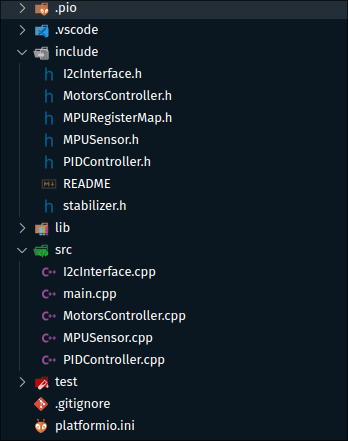
\includegraphics[width=0.25\textwidth]{Figures/folder-structure.png}
	\caption{Structure du Dossier}
	\label{fig:folder-structure}
\end{figure}

\paragraph{L'approche orientée objet est utilisée pour structurer le code en classes. Cela permet de regrouper les fonctions et les variables associées dans des classes, ce qui facilite la gestion et la maintenance du code.}

\paragraph{Diagramme UML des classes :}
\paragraph*{}
\begin{figure}[!htpb]
	\centering
	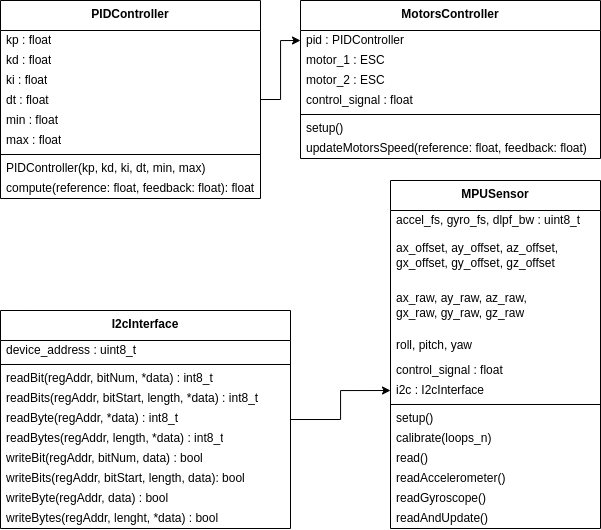
\includegraphics[width=\textwidth]{Figures/uml-oop.png}
	\caption{Diagramme de Classes}
	\label{fig:uml-diagram}
\end{figure}

\subsection{I2cInterface Class}
\paragraph{La classe I2cInterface est utilisée pour communiquer avec les périphériques I2C. Elle contient les fonctions pour lire et écrire des données sur le bus I2C.}
\newpage
\begin{listing}[!htpb]
	\inputminted{cpp}{Code/I2cInterface.h}
	\caption{Classe I2cInterface}
	\label{listing:i2c-interface}
\end{listing}

\paragraph{La fonction la plus pertinente readBytes est utilisée pour lire plusieurs octets à partir d'un registre. Elle prend en entrée l'adresse du registre, le pointeur vers le tampon de données et le nombre d'octets à lire.}
\newpage
\begin{listing}[!htpb]
	\begin{minted}{cpp}
int8_t I2cInterface::readBytes(uint8_t regAddr, uint8_t length, uint8_t *data)
{
	if (length >= BUFFER_LENGTH)
	{
#ifdef DEBUG_LOGS
		Serial.println("I2C error: Uimplemented feature reading more than 32 bytes at once.");
#endif
		return (-1);
	}

	uint8_t count = 0;
	uint32_t initialTime = millis();

	Wire.beginTransmission(deviceAddress);
	Wire.write(regAddr);
	Wire.endTransmission();
	Wire.requestFrom(deviceAddress, length);

	while (Wire.available())
	{
		if (millis() - initialTime >= readTimeout)
		{
#ifdef DEBUG_LOGS
			Serial.println("I2C error: Read Timeout");
#endif
			return (-1);
		}
		data[count++] = Wire.read();
	}

	if (count < length)
	{
#ifdef DEBUG_LOGS
		Serial.println("I2C error: mismatch in read length");
#endif
		return (-1);
	}

	return count;
}
	\end{minted}
	\caption{Implementation de la fonction readBytes}
	\label{listing:read-bytes}
\end{listing}



\subsection{MPUSensor Class}

\paragraph{La classe MPUSensor implemente l'estimateur de l'orientation et utilise La classe I2cInterface pour communiquer avec l'\gls{imu} MPU6050. Elle contient les fonctions pour lire les données de l'\gls{imu}, initialiser la configuration de l'\gls{imu}, calibrer l'\gls{imu}.}
\begin{listing}[!htpb]
	\inputminted{cpp}{Code/MPUSensor.h}
	\caption{Classe MPUSensor}
	\label{listing:mpu-sensor}
\end{listing}


\paragraph{La creation d'objet de la classe MPUSensor est modulaire et reglable en utilisant le constructeur de la classe.}
\paragraph*{Par exemple pour les valeurs suivantes :}
\begin{itemize}
	\item \textbf{Periode d'echantillonnage :} 0.004s
	\item \textbf{Plage de mesure de l'accélération :} $\pm 4g$
	\item \textbf{Plage de mesure de la vitesse angulaire :} $\pm 250^\circ/s$
	\item \textbf{Bande passante du filtre passe-bas :} 42Hz
	\item \textbf{Adresse I2C de l'IMU :} 0x69
\end{itemize}

\begin{listing}[!htpb]
	\begin{minted}{cpp}
/**
 * @brief Create a new MPUSensor object with the specified parameters
 * 
 * @param delta_t Periode d'echantillonnage =  0.004s
 * @param accelRange Accelerometer full scale range = 4g
 * @param gyroRange Gyroscope full scale range = 250°/s
 * @param dlpfBandwidth Digital low pass filter bandwidth = 42Hz
 * @param address I2C address of the MPU6050

 */

 MPUSensor mpu(
	0.004f,
	MPU6050_ACCEL_FS_4,
	MPU6050_GYRO_FS_250,
	MPU6050_DLPF_BW_42,
	MPU6050_ADDRESS_AD0_HIGH
);
	\end{minted}
	\caption{Creation d'objet de la classe MPUSensor}
	\label{listing:mpu-object}
\end{listing}



\paragraph{L'implementation des 3 fonctions pertinentes de la classe MPUSensor est presentée ci-dessous :}
\begin{itemize}
	\item \textbf{setup :} Initialiser la configuration de l'\gls{imu}
	\item \textbf{calibrate :} Calibrer l'\gls{imu}
	\item \textbf{readAndUpdate :} Lire les données de l'\gls{imu} et mettre à jour l'orientation
\end{itemize}
\begin{listing}[!htpb]
	\begin{minted}{cpp}
void MPUSensor::setup()
{
	while (getDeviceId() != MPU6050_WHO_AM_I)
		delay(5000);

#ifdef DEBUG_LOGS
	Serial.println("Successfully Found MPU Sensor ...");
	Serial.println("Configuring MPU Sensor ...");
#endif
	// By default the MPU-6050 sleeps. So we have to wake it up.
	// We want to write to the PWR_MGMT_1 register (6B hex) 0 at SLEEP bit
	if (!i2c.writeBit(MPU6050_RA_PWR_MGMT_1, MPU6050_PWR1_SLEEP_BIT, 0))
	{
#ifdef DEBUG_LOGS
		Serial.println("Error: Could not wake up MPU Sensor.");
#endif
	}
	// Set the Clock Source to PLL with X axis gyroscope reference
	if (!i2c.writeBits(MPU6050_RA_PWR_MGMT_1, MPU6050_PWR1_CLKSEL_BIT, MPU6050_PWR1_CLKSEL_LENGTH, 0x01))
	{
#ifdef DEBUG_LOGS
		Serial.println("Error: Could not set the clock source to PLL with X axis gyroscope reference.");
#endif
	}
	// Set the full scale of the gyro to (default = +- 250º/s).
	if (!i2c.writeBits(MPU6050_RA_GYRO_CONFIG, MPU6050_GCONFIG_FS_SEL_BIT, MPU6050_GCONFIG_FS_SEL_LENGTH, gyro_fs))
	{
#ifdef DEBUG_LOGS
		Serial.println("Error: Could not set the full scale of the gyro.");
#endif
	}
	// Set the full scale of the accelerometer to (default = +- 4g).
	if (!i2c.writeBits(MPU6050_RA_ACCEL_CONFIG, MPU6050_ACONFIG_AFS_SEL_BIT, MPU6050_ACONFIG_AFS_SEL_LENGTH, accel_fs))
	{
#ifdef DEBUG_LOGS
		Serial.println("Error: Could not set the full scale of the accelerometer to +/- 4g.");
#endif
	}
	// Set some filtering to improve the raw data. BandWidth (default = 42Hz)
	if (!i2c.writeBits(MPU6050_RA_CONFIG, MPU6050_CFG_DLPF_BIT, MPU6050_CFG_DLPF_LENGTH, dlpf_bw))
	{
#ifdef DEBUG_LOGS
		Serial.println("Error: Could not set some filtering to improve the raw data.");
#endif
	}
	calibrate(CALIBRATION_LOOP_N);
	delay(1000);
}
	\end{minted}
	\caption{Implementation de la fonction setup de la classe MPUSensor}
	\label{listing:mpu-setup}
\end{listing}

\begin{listing}[!htpb]
	\begin{minted}{cpp}
void MPUSensor::calibrate(uint16_t loops_number)
{
#ifdef DEBUG_LOGS
	Serial.println("-----------------------------------");
	Serial.println("Starting MPU Sensor calibration ...");
#endif
	ax_offset = ay_offset = az_offset = gx_offset = gy_offset = gz_offset = 0;
	uint16_t counter;
	for (counter = 0; counter < loops_number; counter++)
	{
		readAccelerometer(true);
		ax_offset += ax_raw;
		ay_offset += ay_raw;
		az_offset += az_raw;
#ifdef DEBUG_LOGS
		Serial.print(".");
#endif
		delayMicroseconds(3700);
	}
	ax_offset /= loops_number;
	ay_offset /= loops_number;
	az_offset /= loops_number;
#ifdef DEBUG_LOGS
	Serial.println("");
	Serial.println("Accelerometer Calibration done.");
	Serial.println("ax_offset:\t" + String(ax_offset));
	Serial.println("ay_offset:\t" + String(ay_offset));
	Serial.println("az_offset:\t" + String(az_offset));
	Serial.println("Starting Gyroscope Calibration ...");
#endif
	for (counter = 0; counter < loops_number; counter++)
	{
		readGyroscope(true);
		gx_offset += gx_raw;
		gy_offset += gy_raw;
		gz_offset += gz_raw;
#ifdef DEBUG_LOGS
		Serial.print(".");
#endif
		delayMicroseconds(3700);
	}
	gx_offset /= loops_number;
	gy_offset /= loops_number;
	gz_offset /= loops_number;
#ifdef DEBUG_LOGS
	Serial.println("");
	Serial.println("Gyroscope Calibration done.");
	Serial.println("gx_offset:\t" + String(gx_offset));
	Serial.println("gy_offset:\t" + String(gy_offset));
	Serial.println("gz_offset:\t" + String(gz_offset));
	Serial.println("Calibration done.");
#endif
}
	\end{minted}
	\caption{Implementation de la fonction calibrate}
	\label{listing:mpu-calibrate}
\end{listing}

\newpage

\begin{listing}[!htpb]
	\begin{minted}{cpp}
void MPUSensor::readAndUpdate()
{
	read();
	// Roll calculation
	a_roll = atan2(-ay_g, sqrt(ax_g * ax_g + az_g * az_g)) * _r2d;
	g_roll = roll_deg + gx_deg_s * delta_t;
	roll_rad = (roll_deg = _fusion_alpha * g_roll + (1 - _fusion_alpha) * a_roll) / _r2d;
	// Pitch calculation
	a_pitch = atan2(ax_g, sqrt(ay_g * ay_g + az_g * az_g)) * _r2d;
	g_pitch = pitch_deg + gy_deg_s * delta_t;
	roll_rad = (pitch_deg = _fusion_alpha * g_pitch + (1 - _fusion_alpha) * a_pitch) / _r2d;
	// Yaw calculation
	g_yaw = yaw_deg + gz_deg_s * delta_t;
	yaw_rad = (yaw_deg = g_yaw) / _r2d;
}

void MPUSensor::read()
{
	readAccelerometer();
	readGyroscope();
}

void MPUSensor::readAccelerometer(bool is_calibrating = false)
{
	uint8_t buffer[6];
	if (i2c.readBytes(MPU6050_RA_ACCEL_OUT, 6, buffer) != 6)
	{
#ifdef DEBUG_LOGS
		Serial.println("Error: Could not read the accelerometer data.");
#endif
		return;
	}
	ax_raw = ((((int16_t)buffer[0]) << 8) | buffer[1]);
	ay_raw = ((((int16_t)buffer[2]) << 8) | buffer[3]);
	az_raw = ((((int16_t)buffer[4]) << 8) | buffer[5]);
	if (is_calibrating)
		return;

	ax_raw -= ax_offset;
	ay_raw -= ay_offset;
	az_raw -= az_offset + _a_scale[accel_fs];

	ax_g = ax_raw / _a_scale[accel_fs];
	ay_g = ay_raw / _a_scale[accel_fs];
	az_g = az_raw / _a_scale[accel_fs];
}
	\end{minted}
	\caption{Implementation de la fonction readAndUpdate}
	\label{listing:mpu-read-and-update}
\end{listing}

\subsection{PID}

\paragraph{La classe PID est utilisée pour implémenter l'algorithme de contrôle PID. Elle contient les fonctions pour initialiser les paramètres du PID, calculer la commande de contrôle et ajuster les paramètres du PID.}
\paragraph*{}
\begin{listing}[!htpb]
	\inputminted{cpp}{Code/PIDController.h}
	\caption{Classe PID}
	\label{listing:pid}
\end{listing}

\paragraph{La fonction \textbf{compute} est utilisée pour calculer la commande de contrôle en utilisant l'algorithme de contrôle PID. Elle prend en entrée la consigne et la valeur actuelle, et retourne la commande de contrôle.}
\newpage

\begin{listing}[!htpb]
	\begin{minted}{cpp}
float PIDController::compute(const float ref, const float feedback)
{
	float error = ref - feedback;
	/* Proportional error */
	yp_ = kp_ * error;
	/* Derivative error */
	yd_ = kd_ * (error - prev_error) / dt_;
	prev_error = error;
	/* Compute output */
	y_ = yp_ + ki_ * istate_ + yd_;
	/* Saturation and anti-windup */
	if (y_ > max_)
	{
		y_ = max_;
		if (ki_ * error > 0)
			anti_windup_ = 0;
		else
			anti_windup_ = 1;
	}
	else if (y_ < min_)
	{
		y_ = min_;
		if (ki_ * error < 0)
			anti_windup_ = 0;
		else
			anti_windup_ = 1;
	}
	else
		anti_windup_ = 1;
	/* Integrator state */
	istate_ += dt_ * error * anti_windup_;
	return y_;
}
	\end{minted}
	\caption{Implementation de la fonction compute}
	\label{listing:pid-compute}
\end{listing}

\subsection{MotorsController}

\paragraph{La classe MotorsController est utilisée pour contrôler les moteurs. Elle contient les fonctions pour initialiser les moteurs, contrôler la vitesse des moteurs et arrêter les moteurs. elle utilise la classe PID pour commander le moteur.}
\newpage

\begin{listing}[!htpb]
	\inputminted{cpp}{Code/MotorsController.h}
	\caption{Classe MotorController}
	\label{listing:motor-controller}
\end{listing}

\paragraph{La fonction setup est utilisée pour initialiser les moteurs en utilisant la bibliothèque ESC.}

\paragraph{Lafonction update execute le calcul PID et met à jour la vitesse des moteurs.}

\newpage

\begin{listing}[!htpb]
	\begin{minted}{cpp}
void MotorsController::setup()
{

#ifdef DEBUG_LOGS
	Serial.println("Starting motors setup ....");
	Serial.println("Calibrating 1st motor ...");
#endif
	motor1.calib();

#ifdef DEBUG_LOGS
	Serial.println("Calibrating 2nd motor ...");
#endif
	motor2.calib();

#ifdef DEBUG_LOGS
	Serial.println("Successful Motors setup");
#endif
}
	\end{minted}
	\caption{Implementation de la fonction setup}
	\label{listing:motor-setup}
\end{listing}

\begin{listing}[!htpb]
	\begin{minted}{cpp}
void MotorsController::updateMotorsSpeed(float ref_pitch, float pitch)
{
	// Compute the control signal using the PID controller
	control_signal = pid.compute(ref_pitch, pitch);

	// Update motor speeds based on the control signal
	motor1_speed = constrain(MOTORS_MID_SPEED + control_signal - motor1_offset, MOTORS_MIN_SPEED, MOTORS_MAX_SPEED);
	motor2_speed = constrain(MOTORS_MID_SPEED - control_signal - motor2_offset, MOTORS_MIN_SPEED, MOTORS_MAX_SPEED);

	// Update the motors speed
	motor1.speed(motor1_speed);
	motor2.speed(motor2_speed);
}
	\end{minted}
	\caption{Implementation de la fonction updateMotorsSpeed}
	\label{listing:update-motors-speed}
\end{listing}

\newpage

\subsection{Code Arduino}

\begin{listing}[!htpb]
	\begin{minted}{cpp}
#include "stabilizer.h"

const float delta_t = 0.004f;
const uint16_t delta_t_micros = 4000;

const float alpha_fusion = 0.9996f;
uint32_t loop_timer = 0;
const float pitch_ref = 0.0f;

MPUSensor mpuSensor(delta_t);
MotorsController motorsController(delta_t);

void setup()
{
	// Setup the MPU Sensor
	mpuSensor.setup();

	// Setup the motors
	motorsController.setup();

	loop_timer = micros() + delta_t_micros;
}

void loop()
{
	// Read and update the sensor data: output roll, pitch and yaw
	mpuSensor.readAndUpdate();

	// Update the motors speed
	motorsController.updateMotorsSpeed(pitch_ref, mpuSensor.pitch_deg);

	// Wait for the next loop time
	while (micros() < loop_timer)
		;
	loop_timer += delta_t_micros;
}

	\end{minted}
	\caption{Code Arduino}
	\label{listing:arduino-code}
\end{listing}
